\documentclass[a4paper,12pt]{extarticle}

\usepackage[utf8x]{inputenc}
\usepackage[T1,T2A]{fontenc}
\usepackage[russian]{babel}
\usepackage{hyperref}
\usepackage{indentfirst}
\usepackage{listings}
\usepackage{color}
\usepackage{here}
\usepackage{array}
\usepackage{multirow}
\usepackage{graphicx}
\usepackage{caption}
\usepackage{subcaption}
\usepackage{chngcntr}
\usepackage{amsmath}
\usepackage{amssymb}
\usepackage{pgfplots}
\usepackage{pgfplotstable}
\renewcommand{\lstlistingname}{Программа} % заголовок листингов кода

\bibliographystyle{ugost2008ls}

\usepackage{listings}
\lstset{ %
extendedchars=\true,
keepspaces=true,
language=C++,						% choose the language of the code
basicstyle=\scriptsize,		% the size of the fonts that are used for the code
numbers=left,					% where to put the line-numbers
numberstyle=\scriptsize,		% the size of the fonts that are used for the line-numbers
stepnumber=1,					% the step between two line-numbers. If it is 1 each line will be numbered
numbersep=5pt,					% how far the line-numbers are from the code
backgroundcolor=\color{white},	% choose the background color. You must add \usepackage{color}
showspaces=false				% show spaces adding particular underscores
showstringspaces=false,			% underline spaces within strings
showtabs=false,					% show tabs within strings adding particular underscores
frame=single,           		% adds a frame around the code
tabsize=2,						% sets default tabsize to 2 spaces
captionpos=t,					% sets the caption-position to top
breaklines=true,				% sets automatic line breaking
breakatwhitespace=false,		% sets if automatic breaks should only happen at whitespace
escapeinside={\%*}{*)},			% if you want to add a comment within your code
postbreak=\raisebox{0ex}[0ex][0ex]{\ensuremath{\color{red}\hookrightarrow\space}},
texcl=true,
inputpath=fig,                     % директория с листингами
}

\usepackage[left=2cm,right=2cm,
top=2cm,bottom=2cm,bindingoffset=0cm]{geometry}

%% Нумерация картинок по секциям
\usepackage{chngcntr}
\counterwithin{figure}{section}
\counterwithin{table}{section}

%%Точки нумерации заголовков
\usepackage{titlesec}
\titlelabel{\thetitle.\quad}
\usepackage[dotinlabels]{titletoc}

%% Оформления подписи рисунка
\addto\captionsrussian{\renewcommand{\figurename}{Рисунок}}
\captionsetup[figure]{labelsep = period}

%% Подпись таблицы
\DeclareCaptionFormat{hfillstart}{\hfill#1#2#3\par}
\captionsetup[table]{format=hfillstart,labelsep=newline,justification=centering,skip=-10pt,textfont=bf}

%% Путь к каталогу с рисунками
\graphicspath{{fig/}}


\begin{document}	% начало документа

% Титульная страница
\begin{titlepage}	% начало титульной страницы

	\begin{center}		% выравнивание по центру

		\large Санкт-Петербургский Политехнический Университет Петра Великого\\
		\large Институт компьютерных наук и технологий \\
		\large Кафедра компьютерных систем и программных технологий\\[6cm]
		% название института, затем отступ 6см
		
		\huge Вычислительная математика\\[0.5cm] % название работы, затем отступ 0,5см
		\large Отчет по лабораторной работе №1\\[0.1cm]
		\large <<Сравнение точности интерполяционных полиномов>>\\[0.1cm]
		\large Вариант №5\\[5cm]

	\end{center}


	\begin{flushright} % выравнивание по правому краю
		\begin{minipage}{0.25\textwidth} % врезка в половину ширины текста
			\begin{flushleft} % выровнять её содержимое по левому краю

				\large\textbf{Работу выполнил:}\\
				\large Ламтев А.Ю.\\
				\large {Группа:} 23501/4\\
				
				\large \textbf{Преподаватель:}\\
				\large Цыган В.Н.

			\end{flushleft}
		\end{minipage}
	\end{flushright}
	
	\vfill % заполнить всё доступное ниже пространство

	\begin{center}
	\large Санкт-Петербург\\
	\large \the\year % вывести дату
	\end{center} % закончить выравнивание по центру

\thispagestyle{empty} % не нумеровать страницу
\end{titlepage} % конец титульной страницы

\vfill % заполнить всё доступное ниже пространство


\section{Цель работы}
Сравнить точность интерполяционных сплайн-полинома и полинома Лагранжа для заданной функции.

\section{Решаемые задачи}
\begin{enumerate}

\item Для $2 \leq x \leq 3$ с шагом $h = 0.1$ вычислить значение функции f(x) с использованием программы \textbf{QUANC8}, где $f(x) = \int_{0}^{x} \frac{sin(t)}{t} dt$.

\item По полученным точкам построить сплайн-функцию и полином Лагранжа 10-й степени.

\item  В точках $x_k = (k - 0.5) \cdot h + 2$, для $k = 1, 2, \dots, 10$ сравнить значение сплайн-функции и полинома с точным значением f(x), которое вычисляется при помощи \textbf{QUANC8} с высокой точностью.
\end{enumerate}


\section{Ход выполнения работы}

В ходе выполнения работы было разработано программное обеспечение, позволяющее решить поставленные задачи. Исходный код программы представлен в приложении 1.

 На рис. \ref{pic:demo} представлен вывод разработанной программы. В столбце \textbf{x\_k} находятся точки, в которых были посчитаны значения интерполяционного полинома Лагранжа (столбец \textbf{lagrange}), интерполяционного сплайн-полинома (столбец \textbf{spline}) и таблично заданной функции (столбец \textbf{quanc8}).

\begin{figure}[H]
	\begin{center}
		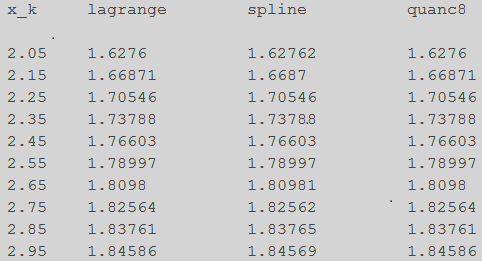
\includegraphics[scale=1]{demo}
		\caption{Результат работы программы} 
		\label{pic:demo} % название для ссылок внутри кода
	\end{center}
\end{figure}

Как видно по выводу программы, значения полинома Лагранжа совпадают с точным значением функции в заданных точках, а значения сплайн-полинома отличаются от точных значений функции в заданных точках.

\section{Выводы}
Из сравнения значений заданной функции со значениями интерполяционных полиномов в определённом наборе точек следует, что интерполяционный полином Лагранжа больше подходит для интерполяции заданной функции, если критерием близости является равенство именно в конкретном определённом наборе точек. Если критерий близости другой, то из полученных данных нельзя сделать вывод о преимуществе одного интерполяционного полинома над другим.

\section*{Приложение 1. Листинги кода} \label{sec:appendix1}

\lstinputlisting[
	label=code:main,
	caption={main.cpp},% для печати символ '_' требует выходной символ '\'
]{../../../app/src/main.cpp}
\parindent=1cm % командна \lstinputlisting сбивает параментры отступа

\lstinputlisting[
	label=code:util,
	caption={util.cpp},% для печати символ '_' требует выходной символ '\'
]{../../../lib/src/util.cpp}
\parindent=1cm % командна \lstinputlisting сбивает параментры отступа

\lstinputlisting[
	label=code:quanc8calculation,
	caption={quanc8\_calculation.cpp},% для печати символ '_' требует выходной символ '\'
]{../../../lib/src/quanc8_calculation.cpp}
\parindent=1cm % командна \lstinputlisting сбивает параментры отступа

\lstinputlisting[
	label=code:lagrangecalculation,
	caption={lagrange\_calculation.cpp},% для печати символ '_' требует выходной символ '\'
]{../../../lib/src/lagrange_calculation.cpp}
\parindent=1cm % командна \lstinputlisting сбивает параментры отступа

\lstinputlisting[
	label=code:splinecalculation,
	caption={spline\_calculation.cpp},% для печати символ '_' требует выходной символ '\'
]{../../../lib/src/spline_calculation.cpp}
\parindent=1cm % командна \lstinputlisting сбивает параментры отступа

\end{document}
